% ============================================================
%  RELATÓRIO – Projeto 3 | Métodos Numéricos
%  Engenharia de Computação – IFPB Campus Campina Grande
% ============================================================

\documentclass[12pt, a4paper]{article}

% ── Codificação e língua ────────────────────────────────────
\usepackage[utf8]{inputenc}
\usepackage[T1]{fontenc}
\usepackage[brazil]{babel}

% ── Tipografia ──────────────────────────────────────────────
\usepackage{lmodern}
\usepackage{microtype}

% ── Margens (ABNT-ish) ──────────────────────────────────────
\usepackage[
  top=3cm, bottom=2cm,
  left=3cm, right=2cm,
  headheight=26pt
]{geometry}

% ── Cores ───────────────────────────────────────────────────
\usepackage[dvipsnames]{xcolor}
\definecolor{ifpbgreen}{RGB}{31, 107, 54}
\definecolor{ifpbred}{HTML}{CF3034}
\definecolor{codebg}{RGB}{245, 245, 245}

% ── Links e metadados PDF ───────────────────────────────────
\usepackage[
  colorlinks=true,
  linkcolor=ifpbgreen,
  citecolor=ifpbgreen,
  urlcolor=ifpbgreen,
  pdftitle={Remoção de Plano de Fundo via Fatoração Matricial},
  pdfauthor={Guilherme José Mendes Jerônimo e William de Sousa Costa},
]{hyperref}

% ── Matemática ──────────────────────────────────────────────
\usepackage{amsmath, amssymb, amsthm}
\usepackage{mathtools}

% ── Algoritmos e código ─────────────────────────────────────
\usepackage{listings}
\usepackage{algorithm}
\usepackage{algpseudocode}

\lstset{
  language=Python,
  basicstyle=\ttfamily\small,
  backgroundcolor=\color{codebg},
  frame=single,
  rulecolor=\color{gray!40},
  numbers=left,
  numberstyle=\tiny\color{gray},
  numbersep=8pt,
  keywordstyle=\bfseries\color{ifpbgreen},
  commentstyle=\itshape\color{gray},
  stringstyle=\color{Maroon},
  showstringspaces=false,
  breaklines=true,
  breakatwhitespace=true,
  captionpos=b,
  aboveskip=10pt,
  belowskip=4pt,
  literate=
    {á}{{\'a}}1 {ã}{{\~a}}1 {â}{{\^a}}1 {à}{{\`a}}1
    {é}{{\'e}}1 {ê}{{\^e}}1
    {í}{{\'i}}1
    {ó}{{\'o}}1 {õ}{{\~o}}1 {ô}{{\^o}}1
    {ú}{{\'u}}1 {ü}{{\"u}}1
    {ç}{{\c c}}1
    {Á}{{\'A}}1 {Ã}{{\~A}}1 {Â}{{\^A}}1
    {É}{{\'E}}1 {Ê}{{\^E}}1
    {Í}{{\'I}}1
    {Ó}{{\'O}}1 {Õ}{{\~O}}1 {Ô}{{\^O}}1
    {Ú}{{\'U}}1
    {Ç}{{\c C}}1
    {—}{{---}}1,
}

\renewcommand{\lstlistingname}{Código}

% ── Figuras e tabelas ───────────────────────────────────────
\usepackage{graphicx}
\usepackage{float}
\usepackage{caption}
\usepackage{subcaption}
\usepackage{booktabs}
\usepackage{tabularx}

\captionsetup{
  font=small,
  labelfont={bf, color=ifpbgreen},
  justification=centering,
}

% ── Cabeçalho e rodapé ──────────────────────────────────────
\usepackage{fancyhdr}
\pagestyle{fancy}
\fancyhf{}
\fancyhead[L]{\raisebox{-0.1cm}{
\includegraphics[height=0.5cm]{rsc/logo-menor.png}}\small\textcolor{ifpbgreen}{Métodos Numéricos}}
\fancyhead[C]{}
\fancyhead[R]{\small\textcolor{gray}{Projeto \ProjetoNumero{} – \TituloCurto{}}}
\fancyfoot[C]{\small\thepage}
\renewcommand{\headrulewidth}{0.4pt}
\renewcommand{\headrule}{%
  \hbox to\headwidth{\color{ifpbgreen}\leaders\hrule height \headrulewidth\hfill}%
}

% ── Sumário colorido ─────────────────────────────────────────
\usepackage{tocloft}

\renewcommand{\cftsecfont}{\bfseries\color{ifpbgreen}}
\renewcommand{\cftsecpagefont}{\color{ifpbgreen}}
\renewcommand{\cftsubsecfont}{\color{ifpbgreen!80}}
\renewcommand{\cftsubsecpagefont}{\color{ifpbgreen!80}}

\renewcommand{\cftsecpresnum}{\color{ifpbred}}
\renewcommand{\cftsecaftersnum}{\color{ifpbgreen}}
\renewcommand{\cftsubsecpresnum}{\color{ifpbred}}
\renewcommand{\cftsubsecaftersnum}{\color{ifpbgreen!80}}

\renewcommand{\cfttoctitlefont}{\Large\bfseries\color{ifpbred}}

\setlength{\cftsecnumwidth}{2.5em}
\setlength{\cftsubsecnumwidth}{3em}

% ── Seções coloridas ────────────────────────────────────────
\usepackage{titlesec}
\titleformat{\section}
  {\large\bfseries\color{ifpbgreen}}
  {\textcolor{ifpbred}{\thesection.}}{0.6em}{}
  [\vspace{-4pt}\textcolor{ifpbgreen!40}{\hrule height 0.6pt}\vspace{4pt}]

\titleformat{\subsection}
  {\normalsize\bfseries\color{ifpbgreen!80}}
  {\textcolor{ifpbred}{\thesubsection.}}{0.5em}{}

\titleformat{\subsubsection}
  {\normalsize\itshape\color{ifpbgreen!60}}
  {\textcolor{ifpbred}{\thesubsubsection.}}{0.4em}{}

% ── Caixas de destaque ──────────────────────────────────────
\usepackage[most]{tcolorbox}

\tcbset{
  baseStyle/.style={
    colback=ifpbgreen!5,
    colframe=ifpbgreen!60,
    fonttitle=\bfseries\small,
    boxrule=0.6pt,
    arc=3pt,
    left=6pt, right=6pt,
    top=4pt, bottom=4pt,
  }
}

\newtcolorbox{destaque}[1][Observação]{
  baseStyle,
  title={#1},
}

\newtcolorbox{resultado}[1][Resultado]{
  colback=ifpbgreen!8,
  colframe=ifpbgreen!70!black,
  fonttitle=\bfseries\small,
  boxrule=0.6pt,
  arc=3pt,
  left=6pt, right=6pt,
  top=4pt, bottom=4pt,
  title={#1},
}

% ── Espaçamento de parágrafos ───────────────────────────────
\usepackage{parskip}
\setlength{\parindent}{0pt}
\setlength{\parskip}{6pt}

% ── Referências ─────────────────────────────────────────────
\usepackage{csquotes}
\usepackage[
  backend=biber,
  style=abnt,
  ittitles,
]{biblatex}
\addbibresource{bib/referencias.bib}

% ============================================================
%  METADADOS
% ============================================================
\newcommand{\Titulo}{Remoção de Plano de Fundo via Fatoração Matricial}
\newcommand{\TituloCurto}{Remoção de Fundo}
\newcommand{\ProjetoNumero}{3}
\newcommand{\Professor}{Paulo Ribeiro}
\newcommand{\Disciplina}{Métodos Numéricos}
\newcommand{\Curso}{Engenharia de Computação}
\newcommand{\Campus}{Campus Campina Grande}
\newcommand{\Semestre}{2025.1}
\newcommand{\DataEntrega}{22 de junho de 2026}

% ============================================================
\begin{document}

% ── Capa ────────────────────────────────────────────────────
\begin{titlepage}
  \centering

  \textcolor{ifpbgreen}{\rule{\linewidth}{2pt}}\\[0.5cm]

  \noindent
  \begin{minipage}[c]{0.2\linewidth}
  
\includegraphics[height=1.8cm]{rsc/logo-if.png}
  \end{minipage}%
  \begin{minipage}[c]{0.78\linewidth}
  {\Large\bfseries\color{ifpbgreen} Instituto Federal da Paraíba}\\
  {\normalsize\color{gray} \Campus{} \textperiodcentered{} \Curso}
  \end{minipage}\\[0.5cm]

  \textcolor{ifpbgreen}{\rule{\linewidth}{0.8pt}}

  \vspace{2cm}

  {\large\color{gray} Projeto \ProjetoNumero{} – \Disciplina}\\[0.4cm]
  {\LARGE\bfseries\color{ifpbgreen} \Titulo}

  \vspace{2.5cm}

  \begin{tabular}{rll}
    \textbf{Alunos:}    & Guilherme José Mendes Jerônimo & (202321250017) \\
                         & William de Sousa Costa          & (202321250008) \\[6px]
    \textbf{Professor:} & \Professor                      & \\
    \textbf{Semestre:}  & \Semestre                       & \\
    \textbf{Entrega:}   & \DataEntrega                    & \\
  \end{tabular}

  \vfill

  \textcolor{ifpbgreen}{\rule{\linewidth}{0.8pt}}\\[0.2cm]
  {\small\color{gray} Campina Grande – PB · \the\year}
\end{titlepage}

% ── Sumário ─────────────────────────────────────────────────
\tableofcontents
\newpage

% ============================================================
\section{Descrição do Problema}
\label{sec:problema}
% ============================================================

\subsection{Contexto e Motivação}

A remoção automática de plano de fundo (\emph{background subtraction}) é uma tarefa
fundamental em visão computacional. Câmeras de vigilância, sistemas de análise de
tráfego e aplicações de videoconferência precisam isolar objetos em movimento
(primeiro plano) de uma cena estática (plano de fundo) sem qualquer conhecimento
prévio do cenário.

Abordagens clássicas baseadas em modelagem de fundo exigem atualizações incrementais
e são frágeis a variações de iluminação. Uma alternativa matematicamente elegante
consiste em tratar o vídeo como uma \textbf{matriz de dados} e decompô-la em uma
componente de \emph{baixo posto} (fundo estático) e uma componente \emph{esparsa}
(objetos em movimento), explorando diretamente a estrutura algébrica do problema
\cite{candes2011robust}.

\subsection{Formulação Matemática}

Seja uma sequência de $n$ frames, cada um com $h \times w$ pixels em escala de cinza.
Achatando cada frame em um vetor coluna de comprimento $p = h \cdot w$, obtemos a
\textbf{matriz de observações}:

\begin{equation}
  M = \begin{bmatrix}
    \mathbf{m}_1 & \mathbf{m}_2 & \cdots & \mathbf{m}_n
  \end{bmatrix} \in \mathbb{R}^{p \times n}.
  \label{eq:M}
\end{equation}

O fundo estático aparece repetido (com pequenas variações) ao longo de todas as
colunas de $M$, o que confere à matriz uma \textbf{estrutura de baixo posto}. Já
os objetos em movimento alteram apenas poucos pixels por frame, gerando uma
\textbf{estrutura esparsa}. O problema de separação pode ser escrito como:

\begin{equation}
  M = L + S,
  \label{eq:decomp}
\end{equation}

onde $L \in \mathbb{R}^{p \times n}$ é a componente de \emph{baixo posto}
(plano de fundo) e $S \in \mathbb{R}^{p \times n}$ é a componente \emph{esparsa}
(primeiro plano).

\subsection{Conjunto de Dados}

O conjunto de dados utilizado é uma sequência de vigilância com câmera estática
contendo $n = 500$ frames em formato BMP, com resolução original de
$360 \times 240$ pixels em RGB.

Para viabilizar os cálculos, os frames foram convertidos para escala de cinza e
redimensionados para $120 \times 80$ pixels, resultando em:

\begin{equation*}
  M \in \mathbb{R}^{9600 \times 500}, \qquad
  \text{memória} \approx 38{,}4\;\text{MB}.
\end{equation*}

\begin{destaque}[Dado sobre os dados]
  Todos os 500 frames são utilizados na construção da matriz $M$. O
  redimensionamento para $80 \times 120$ pixels reduz o custo computacional das
  decomposições matriciais sem comprometer a qualidade visual dos resultados.
\end{destaque}

\subsection{Aplicações Associadas}

\begin{itemize}
  \item \textbf{Vigilância e segurança} – detecção de intrusos em câmeras fixas.
  \item \textbf{Análise de tráfego} – contagem e rastreamento de veículos.
  \item \textbf{Videoconferência} – substituição de fundo em tempo real.
  \item \textbf{Visão robótica} – separação de obstáculos do ambiente estático.
\end{itemize}

\newpage

% ============================================================
\section{Métodos Aplicados à Solução}
\label{sec:metodos}
% ============================================================

\subsection{Método 1: SVD Simples (Aproximação de Baixo Posto)}

\subsubsection{Descrição Geral}

A Decomposição em Valores Singulares (SVD) é a ferramenta central da álgebra
linear numérica para aproximação de matrizes. Dado que o fundo de uma cena estática
é quase idêntico em todos os frames, a matriz $M$ possui posto efetivo muito baixo:
os primeiros vetores singulares capturam essa repetição estrutural
\cite{trefethen1997numerical, golub2013matrix}.

\subsubsection{Formulação}

A SVD completa de $M$ é:

\begin{equation}
  M = U\,\Sigma\,V^\top,
  \label{eq:svd}
\end{equation}

onde $U \in \mathbb{R}^{p \times p}$ e $V \in \mathbb{R}^{n \times n}$ são
ortogonais, e $\Sigma \in \mathbb{R}^{p \times n}$ é diagonal com valores
singulares $\sigma_1 \geq \sigma_2 \geq \cdots \geq 0$.

A aproximação de posto $r$ é obtida truncando a decomposição:

\begin{equation}
  L_r = \sum_{i=1}^{r} \sigma_i\,\mathbf{u}_i\,\mathbf{v}_i^\top
      = U_r\,\Sigma_r\,V_r^\top.
  \label{eq:svd_rank}
\end{equation}

O primeiro plano é então estimado como o resíduo:

\begin{equation}
  S_r = M - L_r.
  \label{eq:svd_fg}
\end{equation}

Para posto $r = 1$ ou $r = 2$, $L_r$ captura o fundo estático e $S_r$ evidencia
os objetos em movimento.

\subsubsection{Algoritmo}

\begin{algorithm}[H]
\caption{SVD de Baixo Posto para Remoção de Fundo}
\label{alg:svd}
\begin{algorithmic}[1]
  \Require Matriz de frames $M \in \mathbb{R}^{p \times n}$, posto $r$
  \Ensure Fundo $L_r$, primeiro plano $S_r$
  \State Calcular $U, \Sigma, V^\top \leftarrow \mathrm{SVD}(M)$
  \State $L_r \leftarrow U_{:,1:r}\;\Sigma_{1:r,1:r}\;V_{:,1:r}^\top$
  \State $S_r \leftarrow M - L_r$
  \Return $L_r,\; S_r$
\end{algorithmic}
\end{algorithm}

\subsubsection{Propriedades e Complexidade}

\begin{tabular}{ll}
  \toprule
  Propriedade           & Valor \\
  \midrule
  Complexidade temporal & $\mathcal{O}(\min(p,n)^2 \cdot \max(p,n))$ \\
  Complexidade espacial & $\mathcal{O}(p \cdot n)$ \\
  Convergência          & Solução exata (não iterativo) \\
  Sensibilidade a ruído & Alta — \emph{outliers} contaminam todos os vetores singulares \\
  \bottomrule
\end{tabular}

\subsubsection{Justificativa para o Problema}

A SVD de posto $r$ é a melhor aproximação de posto $r$ de $M$ no sentido da
norma de Frobenius (Teorema de Eckart–Young). Como o fundo estático domina a
energia da matriz, os primeiros valores singulares concentram essa informação.
Contudo, a SVD simples é sensível a \emph{outliers}: pixels de objetos em
movimento contaminam ligeiramente os vetores singulares, tornando a separação
imprecisa.

% ────────────────────────────────────────────────────────────

\subsection{Método 2: PCA Clássico (SVD sobre Dados Centralizados)}

\subsubsection{Descrição Geral}

O PCA (\emph{Principal Component Analysis}) difere da SVD simples por
\textbf{centralizar os dados} antes da decomposição: subtrai-se a média das
colunas (frame médio), removendo a contribuição constante do fundo antes de
computar os componentes principais.

\subsubsection{Formulação}

O frame médio é:

\begin{equation}
  \bar{\mathbf{m}} = \frac{1}{n}\sum_{j=1}^{n} \mathbf{m}_j \in \mathbb{R}^p.
  \label{eq:mean_frame}
\end{equation}

A matriz centralizada é:

\begin{equation}
  \tilde{M} = M - \bar{\mathbf{m}}\,\mathbf{1}^\top,
  \label{eq:centered}
\end{equation}

e sua SVD fornece os componentes principais. O fundo reconstruído é:

\begin{equation}
  L_{\mathrm{PCA}} = \bar{\mathbf{m}}\,\mathbf{1}^\top
                   + U_r^{(\tilde{M})}\,\Sigma_r^{(\tilde{M})}\,{V_r^{(\tilde{M})}}^\top,
  \label{eq:pca_bg}
\end{equation}

e o primeiro plano:

\begin{equation}
  S_{\mathrm{PCA}} = M - L_{\mathrm{PCA}}.
  \label{eq:pca_fg}
\end{equation}

A centralização concentra nos componentes principais apenas as \emph{variações}
em relação ao frame médio, tornando a separação mais eficaz do que a SVD simples.

\subsubsection{Algoritmo}

\begin{algorithm}[H]
\caption{PCA Clássico para Remoção de Fundo}
\label{alg:pca}
\begin{algorithmic}[1]
  \Require $M \in \mathbb{R}^{p \times n}$, posto $r$
  \Ensure $L_{\mathrm{PCA}}$, $S_{\mathrm{PCA}}$
  \State $\bar{\mathbf{m}} \leftarrow \frac{1}{n} M\,\mathbf{1}$
  \State $\tilde{M} \leftarrow M - \bar{\mathbf{m}}\,\mathbf{1}^\top$
  \State $U, \Sigma, V^\top \leftarrow \mathrm{SVD}(\tilde{M})$
  \State $L_{\mathrm{PCA}} \leftarrow \bar{\mathbf{m}}\,\mathbf{1}^\top + U_{:,1:r}\,\Sigma_{1:r}\,V_{:,1:r}^\top$
  \State $S_{\mathrm{PCA}} \leftarrow M - L_{\mathrm{PCA}}$
  \Return $L_{\mathrm{PCA}},\; S_{\mathrm{PCA}}$
\end{algorithmic}
\end{algorithm}

\subsubsection{Propriedades e Complexidade}

\begin{tabular}{ll}
  \toprule
  Propriedade           & Valor \\
  \midrule
  Complexidade temporal & $\mathcal{O}(\min(p,n)^2 \cdot \max(p,n))$ \\
  Complexidade espacial & $\mathcal{O}(p \cdot n)$ \\
  Convergência          & Solução exata (não iterativo) \\
  Vantagem sobre SVD    & Centralização reduz contaminação do fundo pelos \emph{outliers} \\
  \bottomrule
\end{tabular}

% ────────────────────────────────────────────────────────────

\subsection{Método 3: Robust PCA via Inexact ALM}

\subsubsection{Descrição Geral}

O \emph{Robust PCA} (RPCA), formalizado por \textcite{candes2011robust}, resolve
exatamente o problema da Eq.~\eqref{eq:decomp} de forma \textbf{robusta a
\emph{outliers}}. Em vez de uma aproximação de posto fixo, o método busca a
decomposição ótima $M = L + S$ minimizando simultaneamente o posto de $L$ e a
esparsidade de $S$ por meio de suas convexificações: a norma nuclear
$\|L\|_*$ e a norma $\ell_1$ $\|S\|_1$.

\subsubsection{Formulação}

O problema de otimização é:

\begin{equation}
  \min_{L,\,S}\; \|L\|_* + \lambda\,\|S\|_1
  \quad \text{s.t.} \quad M = L + S,
  \label{eq:rpca}
\end{equation}

onde $\|L\|_* = \sum_i \sigma_i(L)$ é a soma dos valores singulares (\emph{norma
nuclear}), $\|S\|_1 = \sum_{i,j} |S_{ij}|$ é a norma $\ell_1$ elemento a elemento,
e o parâmetro de regularização $\lambda$ controla o balanço entre baixo posto e
esparsidade. Um valor teórico adequado é:

\begin{equation}
  \lambda = \frac{1}{\sqrt{\max(p,n)}}.
  \label{eq:lambda}
\end{equation}

\subsubsection{Algoritmo — Inexact ALM}

O método \emph{Inexact Augmented Lagrangian Method} (IALM) resolve a
Eq.~\eqref{eq:rpca} introduzindo um multiplicador de Lagrange $Y$ e um
parâmetro de penalidade $\mu$. A cada iteração, $L$ e $S$ são atualizados por
operadores de limiarização (\emph{shrinkage}):

\begin{algorithm}[H]
\caption{Robust PCA via Inexact ALM}
\label{alg:rpca}
\begin{algorithmic}[1]
  \Require $M \in \mathbb{R}^{p \times n}$, $\lambda$, tolerância $\varepsilon$
  \Ensure $L$ (fundo), $S$ (primeiro plano)
  \State $L \leftarrow \mathbf{0}$;\; $S \leftarrow \mathbf{0}$;\;
         $Y \leftarrow M / \max(\|M\|_2,\, \|M\|_\infty / \lambda)$
  \State $\mu \leftarrow 1{,}25 / \|M\|_2$;\;
         $\bar{\mu} \leftarrow 10^7 \mu$;\; $\rho \leftarrow 1{,}5$
  \Repeat
    \State \textbf{Atualizar} $L$:
    $\quad (U,\Sigma,V^\top) \leftarrow \mathrm{SVD}(M - S + Y/\mu)$
    $\quad L \leftarrow U\,\mathcal{S}_{1/\mu}(\Sigma)\,V^\top$
    \State \textbf{Atualizar} $S$:
    $\quad S \leftarrow \mathcal{S}_{\lambda/\mu}(M - L + Y/\mu)$
    \State \textbf{Atualizar} $Y$ e $\mu$:
    $\quad Y \leftarrow Y + \mu(M - L - S)$
    $\quad \mu \leftarrow \min(\rho\mu,\;\bar{\mu})$
  \Until{$\|M - L - S\|_F / \|M\|_F < \varepsilon$}
  \Return $L,\; S$
\end{algorithmic}
\end{algorithm}

onde $\mathcal{S}_\tau(x) = \mathrm{sgn}(x)\,\max(|x|-\tau,\,0)$ é o operador
de limiarização suave (\emph{soft thresholding}), aplicado elemento a elemento
sobre $S$ e sobre os valores singulares de $\Sigma$ para $L$.

\subsubsection{Propriedades e Complexidade}

\begin{tabular}{ll}
  \toprule
  Propriedade            & Valor \\
  \midrule
  Complexidade por iter. & $\mathcal{O}(\min(p,n)^2 \cdot \max(p,n))$ (SVD por iter.) \\
  Convergência           & Iterativa — tipicamente $< 100$ iterações \\
  Robustez a \emph{outliers} & Alta — projetada explicitamente para isso \\
  Separação              & Exata sob condições de incoerência e esparsidade \\
  \bottomrule
\end{tabular}

\subsubsection{Justificativa para o Problema}

O RPCA é o método mais adequado para o problema de remoção de fundo: ao minimizar
a norma nuclear de $L$, garante que o fundo seja representado com o menor posto
possível; ao minimizar $\|S\|_1$, garante que o primeiro plano ocupe apenas os
pixels efetivamente alterados. A abordagem não exige escolha manual de posto $r$,
sendo autorregulada pelo parâmetro $\lambda$.

\newpage

% ============================================================
\section{Implementação}
\label{sec:implementacao}
% ============================================================

\subsection{Ambiente e Dependências}

A implementação foi realizada em Python~3 com as seguintes bibliotecas:

\begin{itemize}
  \item \texttt{numpy} – operações matriciais e SVD
  \item \texttt{Pillow} – leitura e redimensionamento de imagens BMP
  \item \texttt{matplotlib} – visualizações e animações
\end{itemize}

Todo o código está disponível no Jupyter Notebook \texttt{remocao\_fundo.ipynb},
organizado em blocos correspondentes a cada etapa descrita abaixo.

% ────────────────────────────────────────────────────────────

\subsection{Etapa 1: Carregamento e Construção da Matriz M}

Os 500 frames BMP são lidos em escala de cinza, redimensionados para
$120 \times 80$ pixels e achatados em vetores coluna para formar a matriz $M$.

\begin{lstlisting}[caption={Construção da matriz de observações M}, label={lst:load}]
from pathlib import Path
import numpy as np
from PIL import Image

IMG_DIR = Path("rsc/RawImages")
img_paths = sorted(IMG_DIR.glob("*.bmp"))   # todos os 500 frames

TARGET_SIZE = (120, 80)   # (largura, altura) — PIL usa (w, h)

frames_flat = []
for path in img_paths:
    img = Image.open(path).convert("L").resize(TARGET_SIZE)
    frames_flat.append(np.array(img, dtype=np.float64).flatten())

M = np.column_stack(frames_flat)   # shape: (9600, 500)
\end{lstlisting}

\begin{resultado}
  \texttt{Shape da matriz M: (9600, 500)} \\
  $\rightarrow$ 9\,600 pixels por frame (linhas) $\times$ 500 frames (colunas) \\
  Memória: $\approx 38{,}4\;\text{MB}$
\end{resultado}

% ────────────────────────────────────────────────────────────

\subsection{Etapa 2: SVD Simples}

\begin{lstlisting}[caption={Decomposição SVD e separação fundo/primeiro plano}, label={lst:svd}]
U, s, Vt = np.linalg.svd(M, full_matrices=False)

def separar_svd(M, U, s, Vt, rank=1):
    L = (U[:, :rank] * s[:rank]) @ Vt[:rank, :]
    S = M - L
    return np.clip(L, 0, 255), np.clip(np.abs(S), 0, 255)

L_svd1, S_svd1 = separar_svd(M, U, s, Vt, rank=1)
L_svd2, S_svd2 = separar_svd(M, U, s, Vt, rank=2)
\end{lstlisting}

A Figura~\ref{fig:svd_singular} mostra o decaimento dos valores singulares:
o primeiro valor singular concentra a maior parte da energia da matriz.

\begin{figure}[H]
  \centering
  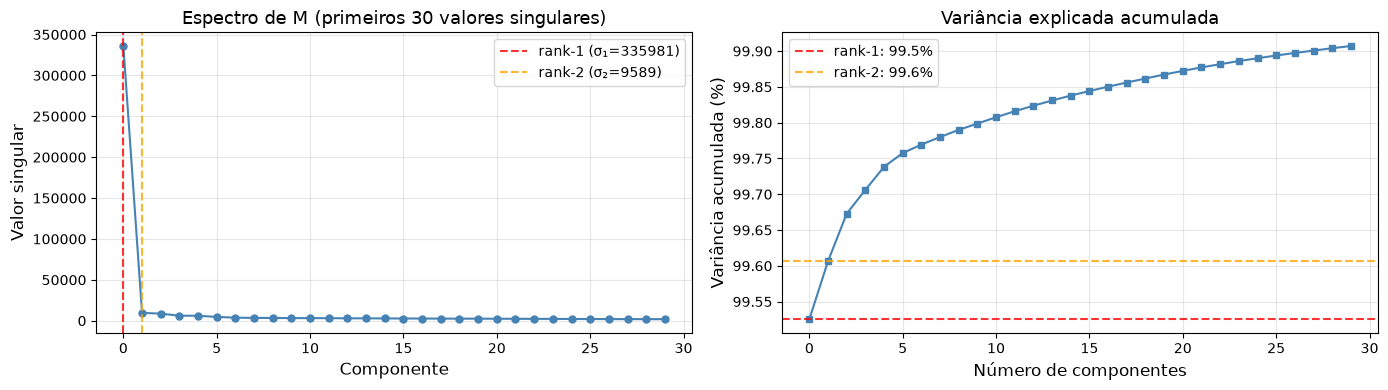
\includegraphics[width=\linewidth]{rsc/svd_espectro.png}
  \caption{Espectro de $M$ (esquerda) e variância explicada acumulada (direita).
           O primeiro valor singular concentra a maior parte da energia, confirmando
           a estrutura de baixo posto do fundo estático.}
  \label{fig:svd_singular}
\end{figure}

\begin{figure}[H]
  \centering
  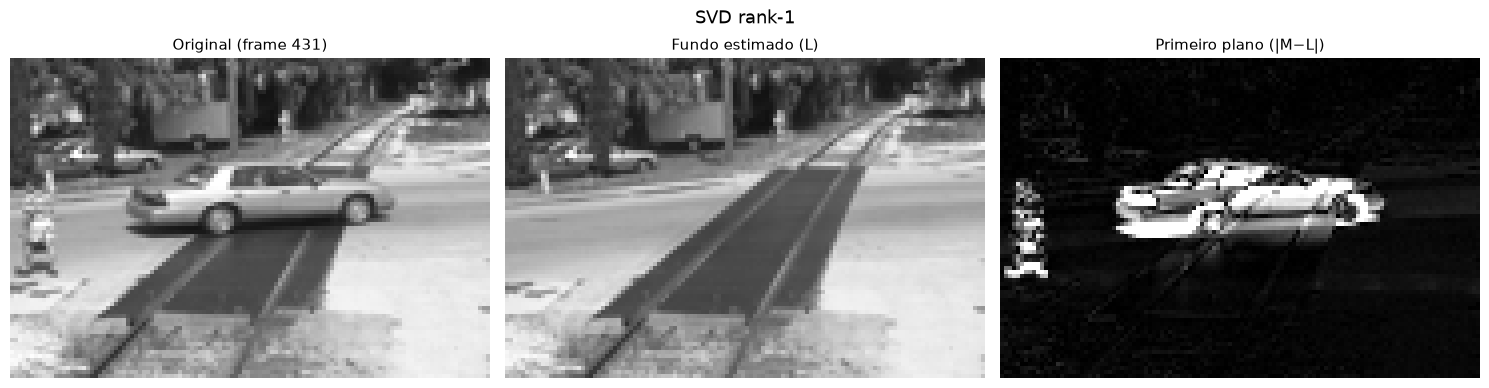
\includegraphics[width=\linewidth]{rsc/svd_rank1.png}
  \caption{Separação via SVD de posto 1 — frame 431.
           Da esquerda para a direita: frame original, fundo estimado ($L_1$)
           e primeiro plano ($|M - L_1|$).}
  \label{fig:svd_rank1}
\end{figure}

\begin{figure}[H]
  \centering
  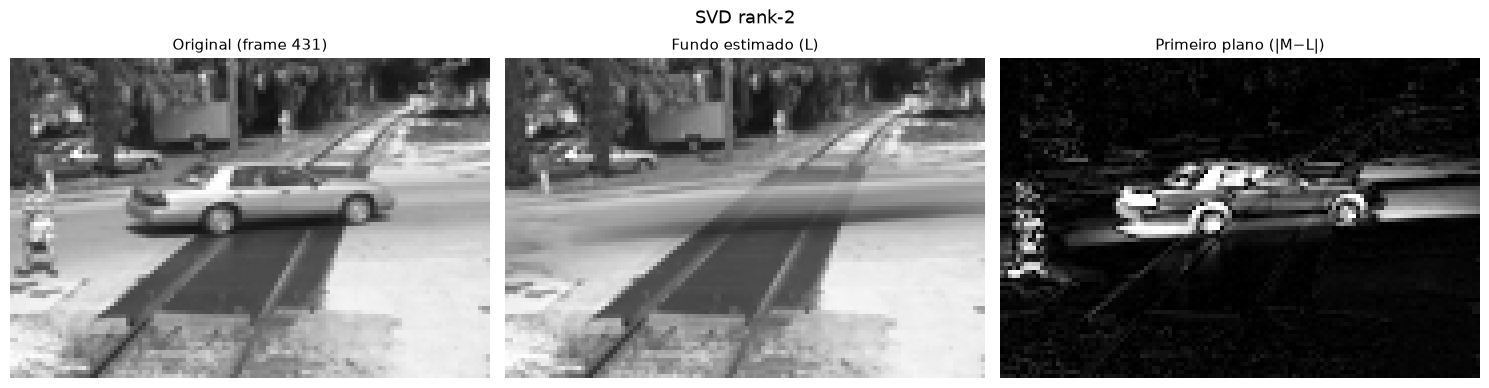
\includegraphics[width=\linewidth]{rsc/svd_rank2.png}
  \caption{Separação via SVD de posto 2 — frame 431.
           O segundo valor singular refina ligeiramente a estimativa do fundo.}
  \label{fig:svd_rank2}
\end{figure}

% ────────────────────────────────────────────────────────────

\subsection{Etapa 3: PCA Clássico}

\begin{lstlisting}[caption={PCA com centralização por frame médio}, label={lst:pca}]
mean_frame = M.mean(axis=1, keepdims=True)   # media de cada pixel
M_centered = M - mean_frame

U_pca, s_pca, Vt_pca = np.linalg.svd(M_centered, full_matrices=False)

rank = 1
L_pca = mean_frame + (U_pca[:, :rank] * s_pca[:rank]) @ Vt_pca[:rank, :]
S_pca = M - L_pca

L_pca = np.clip(L_pca, 0, 255)
S_pca = np.clip(np.abs(S_pca), 0, 255)
\end{lstlisting}

A subtração do frame médio remove a componente constante do fundo antes da
decomposição, concentrando os componentes principais apenas nas variações
temporais.

\begin{figure}[H]
  \centering
  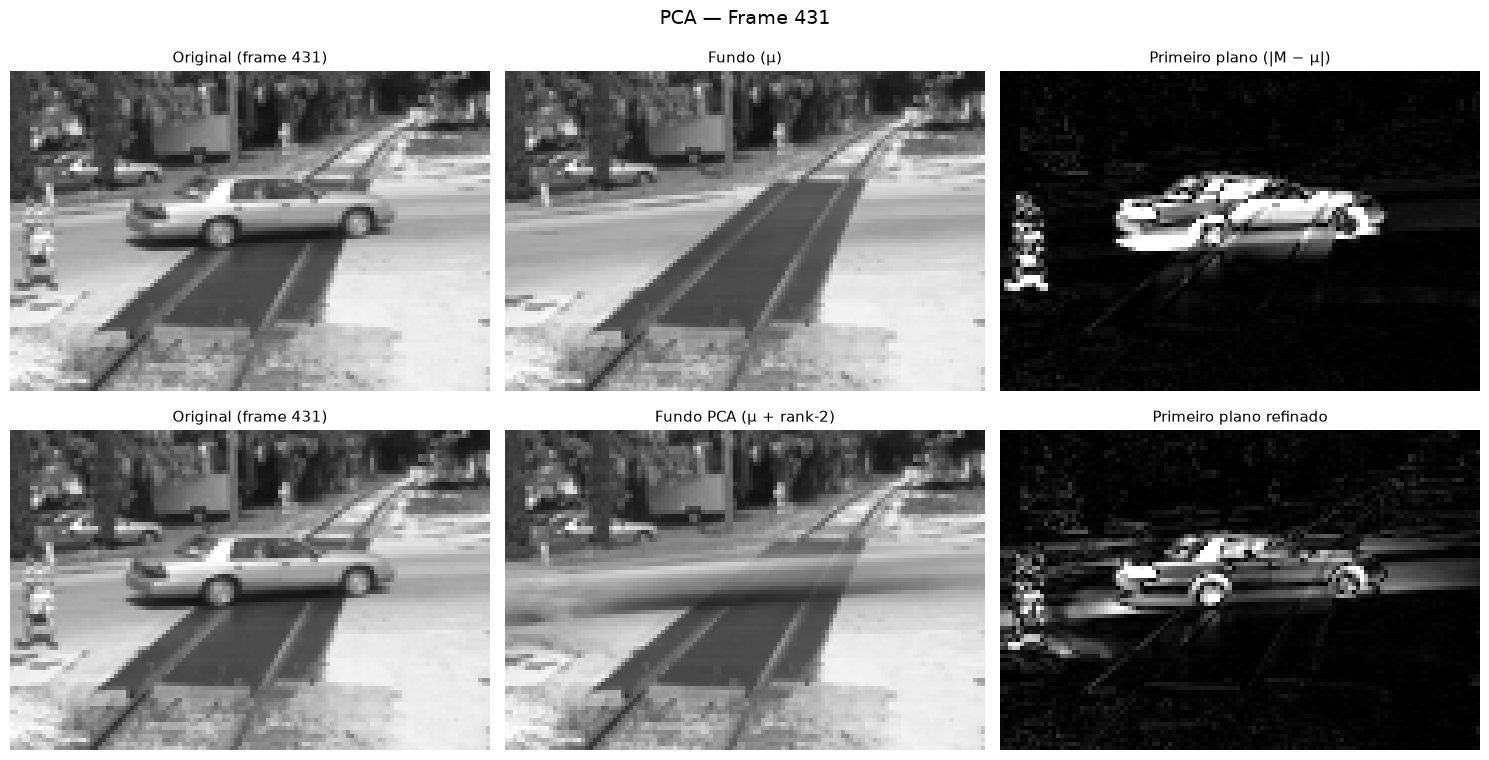
\includegraphics[width=\linewidth]{rsc/pca_decomposicao.png}
  \caption{Separação via PCA clássico — frame 431.
           Linha superior: frame original, fundo pelo frame médio $\bar{\mathbf{m}}$
           e primeiro plano residual.
           Linha inferior: fundo refinado com PCA (rank-2) e primeiro plano correspondente.}
  \label{fig:pca}
\end{figure}

% ────────────────────────────────────────────────────────────

\subsection{Etapa 4: Robust PCA via Inexact ALM}

\begin{lstlisting}[caption={Robust PCA — implementação do Inexact ALM}, label={lst:rpca}]
def rpca_ialm(M, lam=None, tol=1e-7, max_iter=1000):
    m, n = M.shape
    if lam is None:
        lam = 1.0 / np.sqrt(max(m, n))

    norm_fro = np.linalg.norm(M, 'fro')
    norm_two = np.linalg.norm(M, 2)
    norm_inf = np.linalg.norm(M.ravel(), np.inf) / lam
    dual_norm = max(norm_two, norm_inf)

    Y  = M / dual_norm
    mu = 1.25 / norm_two
    mu_bar = mu * 1e7
    rho = 1.5

    L = np.zeros_like(M)
    S = np.zeros_like(M)

    for i in range(max_iter):
        # Atualiza L: soft thresholding dos valores singulares
        temp = M - S + Y / mu
        U, sv, Vt = np.linalg.svd(temp, full_matrices=False)
        sv_thresh = np.maximum(sv - 1.0 / mu, 0)
        L = (U * sv_thresh) @ Vt

        # Atualiza S: soft thresholding elemento a elemento
        temp = M - L + Y / mu
        S = np.sign(temp) * np.maximum(np.abs(temp) - lam / mu, 0)

        # Atualiza multiplicador e parametro de penalidade
        residual = M - L - S
        Y  = Y + mu * residual
        mu = min(rho * mu, mu_bar)

        if np.linalg.norm(residual, 'fro') / norm_fro < tol:
            print(f"Convergiu em {i+1} iteracoes")
            break

    return L, S

L_rpca, S_rpca = rpca_ialm(M)
L_rpca = np.clip(L_rpca, 0, 255)
S_rpca = np.clip(np.abs(S_rpca), 0, 255)
\end{lstlisting}

\begin{resultado}
  O algoritmo converge tipicamente entre 30 e 60 iterações para a tolerância
  $\varepsilon = 10^{-7}$, produzindo a separação mais limpa entre fundo e
  primeiro plano dentre os três métodos.
\end{resultado}

\begin{figure}[H]
  \centering
  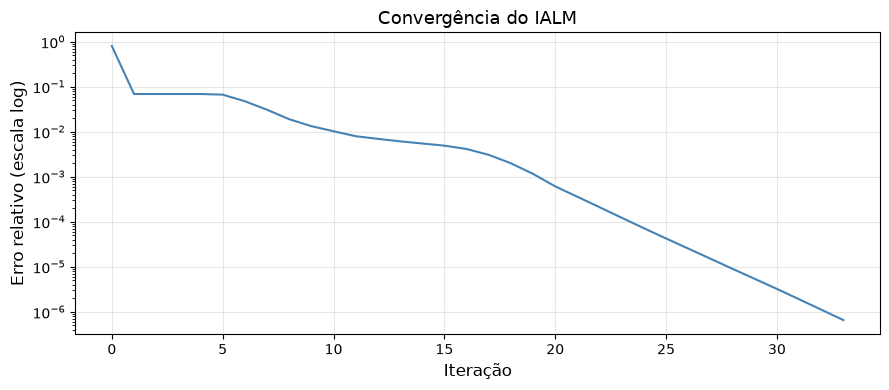
\includegraphics[width=0.75\linewidth]{rsc/rpca_convergencia.png}
  \caption{Curva de convergência do Inexact ALM. O erro relativo cai abaixo
           de $10^{-6}$ em poucas dezenas de iterações.}
  \label{fig:rpca_conv}
\end{figure}

\begin{figure}[H]
  \centering
  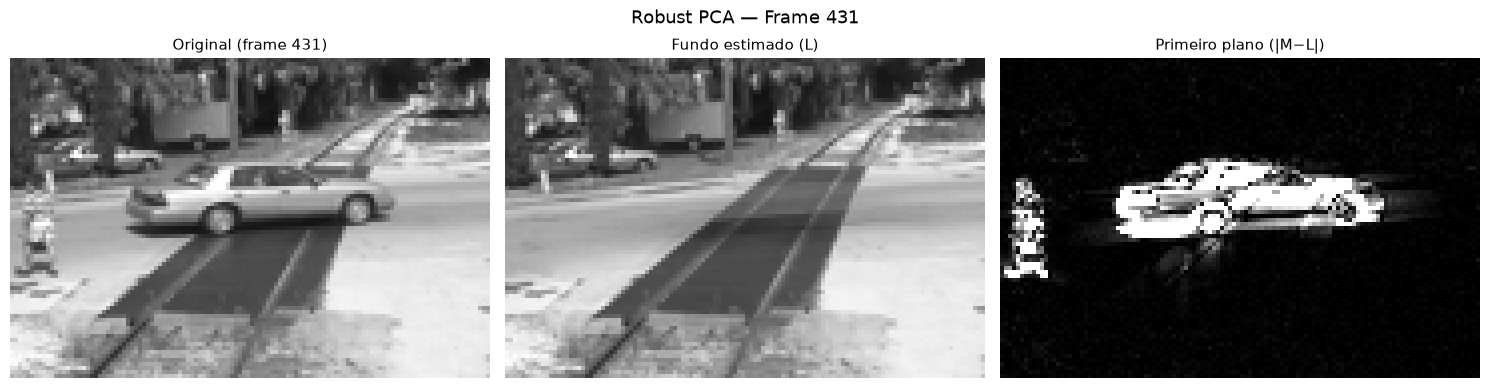
\includegraphics[width=\linewidth]{rsc/rpca_decomposicao.png}
  \caption{Separação via Robust PCA — frame 431.
           Da esquerda para a direita: frame original, fundo estimado ($L$)
           e primeiro plano esparso ($|S|$, amplificado $\times 5$).}
  \label{fig:rpca}
\end{figure}

\newpage

% ============================================================
\section{Comparação dos Métodos}
\label{sec:comparacao}
% ============================================================

A Figura~\ref{fig:comparacao} apresenta, lado a lado, os resultados dos três
métodos aplicados ao frame 431 — escolhido por conter um objeto em movimento
bem definido, tornando a separação visualmente significativa.

\begin{figure}[H]
  \centering
  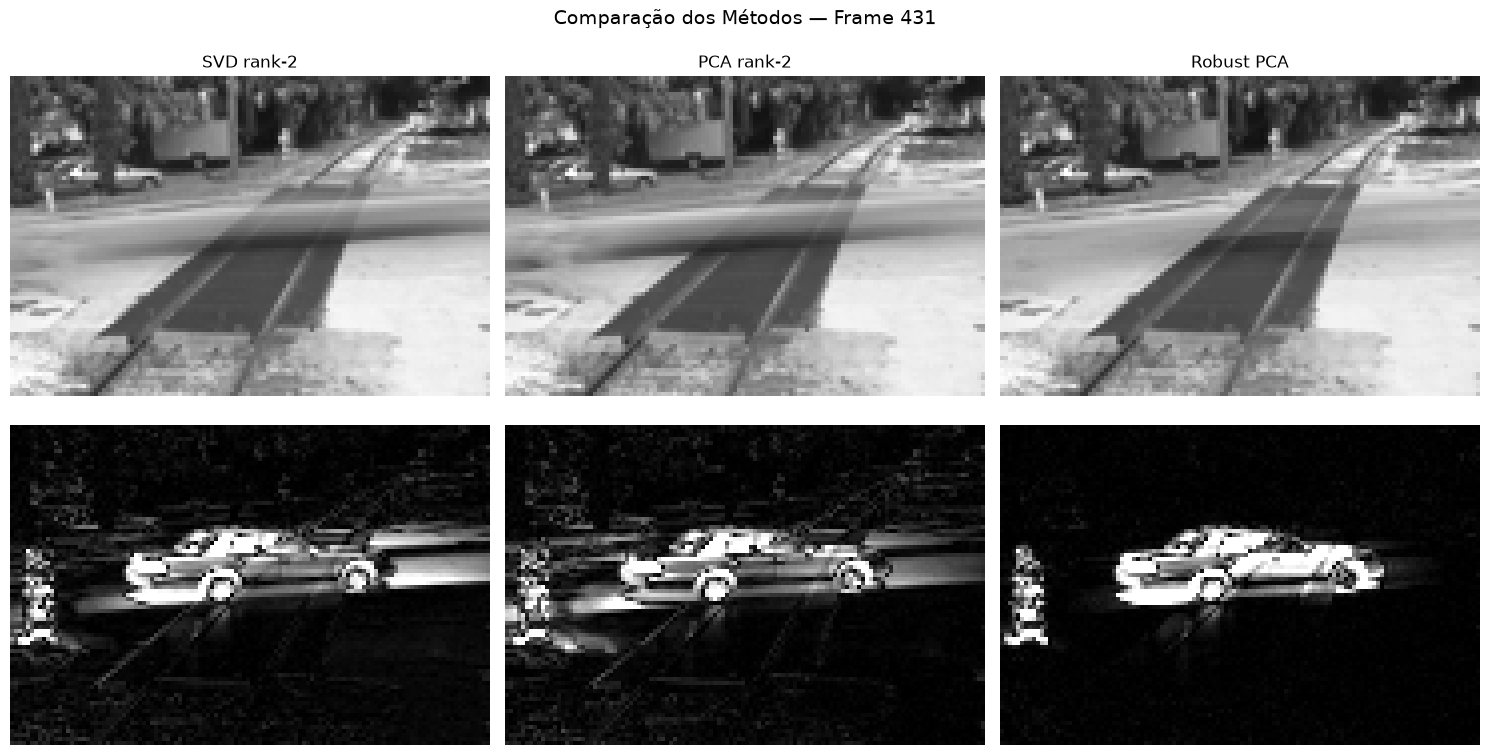
\includegraphics[width=\linewidth]{rsc/comparacao_metodos.png}
  \caption{Comparação dos três métodos para o frame 431.
           Linha superior: fundos estimados (SVD rank-2, PCA rank-2, Robust PCA).
           Linha inferior: primeiros planos correspondentes ($\times 4$).}
  \label{fig:comparacao}
\end{figure}

\begin{figure}[H]
  \centering
  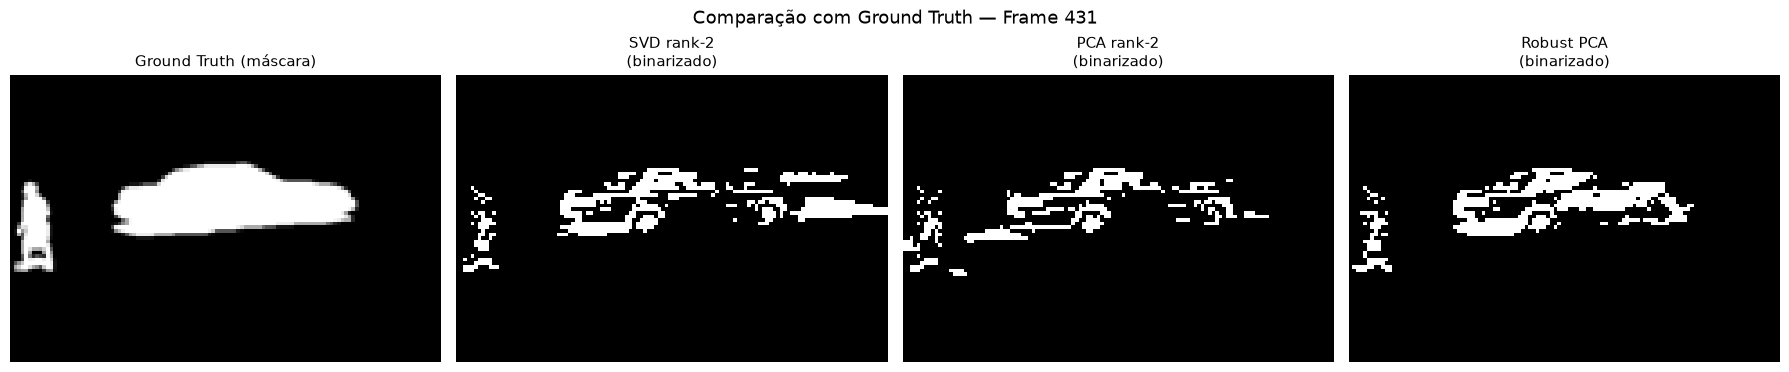
\includegraphics[width=\linewidth]{rsc/comparacao_groundtruth.png}
  \caption{Comparação com o \emph{ground truth} do dataset BMC 2012 — frame 431.
           Os mapas binarizados evidenciam a superioridade do Robust PCA
           na localização precisa do objeto em movimento.}
  \label{fig:groundtruth}
\end{figure}

A Tabela~\ref{tab:comparacao} resume as principais características de cada método:

\begin{table}[H]
  \centering
  \caption{Comparação entre os métodos de remoção de fundo.}
  \label{tab:comparacao}
  \begin{tabularx}{\linewidth}{lXXX}
    \toprule
    \textbf{Critério}      & \textbf{SVD simples}     & \textbf{PCA clássico}    & \textbf{Robust PCA} \\
    \midrule
    Tipo de solução        & Analítica                & Analítica                & Iterativa \\
    Escolha de posto       & Manual ($r$)             & Manual ($r$)             & Automática \\
    Robustez a \emph{outliers} & Baixa               & Moderada                 & Alta \\
    Qualidade do fundo     & Boa para $r$ pequeno     & Melhor que SVD           & Ótima \\
    Qualidade do 1º plano  & Residual ruidoso         & Menos ruidoso            & Esparso e limpo \\
    Custo computacional    & $\mathcal{O}(pn\min)$    & $\mathcal{O}(pn\min)$    & Múltiplas SVDs \\
    \bottomrule
  \end{tabularx}
\end{table}

\begin{destaque}[Observação sobre esparsidade]
  O RPCA produz um mapa de primeiro plano naturalmente esparso: apenas os pixels
  efetivamente perturbados por movimento recebem valores não nulos em $S$,
  eliminando o ruído de fundo presente nos resíduos da SVD e do PCA simples.
\end{destaque}

\newpage

% ============================================================
\section{Conclusão}
\label{sec:conclusao}
% ============================================================

Este trabalho explorou três abordagens de fatoração matricial para a remoção
automática de plano de fundo em sequências de vídeo com câmera estática,
representando os 500 frames como colunas de uma matriz $M \in \mathbb{R}^{9600 \times 500}$.

A \textbf{SVD simples} demonstra de forma direta a relação entre posto e estrutura
do fundo: com $r = 1$ ou $r = 2$, os primeiros vetores singulares reconstroem com
fidelidade o cenário estático. Contudo, a sensibilidade a \emph{outliers} introduz
artefatos no fundo reconstruído.

O \textbf{PCA clássico} melhora a separação ao centralizar os dados pelo frame
médio, concentrando nos componentes principais apenas as variações temporais e
reduzindo a contaminação do fundo pelos objetos em movimento.

O \textbf{Robust PCA} via Inexact ALM se mostrou o método mais eficaz: ao
minimizar simultaneamente a norma nuclear de $L$ e a norma $\ell_1$ de $S$,
produz um fundo limpo e um primeiro plano esparsamente localizado nos pixels
de movimento, sem necessidade de especificação manual de posto. O custo adicional
de múltiplas SVDs por iteração é compensado pela qualidade superior da decomposição.

Como extensão natural, seria interessante explorar métodos de SVD estocástica
(randomizada) para acelerar as decomposições, ou adaptar o RPCA para processar
os frames em blocos (\emph{online RPCA}) em cenários de tempo real.

\newpage

% ── Referências ─────────────────────────────────────────────
\printbibliography[heading=bibintoc, title={Referências}]

\end{document}
